\documentclass[xcolor={dvipsnames}]{beamer}
\usepackage{color, colortbl}
\usepackage{transparent}
\usepackage[ngerman,english]{babel}
\usepackage[T1]{fontenc}
\usepackage{lmodern}
%\usepackage{subfigure}
%\usepackage[compatibility=false]{caption}
%\usepackage{subcaption}
\usepackage{tikz}
\usepackage{textgreek}
\usepackage{tabularx}
\usepackage{booktabs}
\usepackage{siunitx}
\usepackage{units}
\usepackage[absolute,overlay]{textpos} %for positioning the logos where I want

\mode<presentation>
{
  \usetheme{CambridgeUS}     
  \usecolortheme{lily} 
  \definecolor{beamer@violet}{rgb}{0.5,0.3,0.5} % changed this
  \setbeamercolor{structure}{fg=beamer@violet!70!cyan}
  \setbeamercolor{palette primary}{fg=black, bg=gray!30!white!50!cyan!20!}
  \setbeamercolor{palette secondary}{fg=black, bg=gray!30!white!30!cyan!40!}
  \setbeamercolor*{palette tertiary}{bg=gray!20!white!20!cyan!60!}
  
  \setbeamercolor{frametitle}{fg=cyan!60!white!40!,bg=cyan!80!black}
  \setbeamercolor{title}{fg=cyan!80!black}
  \setbeamercolor{normal text}{fg=black,bg=white}
  \setbeamercolor{alerted text}{fg=beamer@violet}
  \setbeamercolor{example text}{fg=beamer@violet!70!cyan}
  
  \usefonttheme{structureitalicserif} 
  \setbeamertemplate{navigation symbols}{}
  \setbeamertemplate{caption}[numbered]
} 

\newcommand{\sidlogo}{
  \setlength{\TPHorizModule}{1pt}
  \setlength{\TPVertModule}{1pt}
   % textblock{}{x,y}: pos(x) = rightUpperCorner + (x * \TPHorizModule), pos(y) = leftUpperCorner - (y * \TPVertModule)
  \begin{textblock}{1}(323,12)
   
\includegraphics[width=40pt,height=26pt]{figures/SiD.jpeg}
  \end{textblock}
  } 
\newcommand{\ilclogo}{
  \setlength{\TPHorizModule}{1pt}
  \setlength{\TPVertModule}{1pt}
   % textblock{}{x,y}: pos(x) = rightUpperCorner + (x * \TPHorizModule), pos(y) = leftUpperCorner - (y * \TPVertModule)
  \begin{textblock}{1}(323,12)
   
\includegraphics[width=40pt,height=26pt]{figures/ILC.jpeg}
  \end{textblock}
} 

\title[ILC \& Muons from spoilers]{\textbf{\LARGE Muon background from the BDS\\in SiD} \\ \vspace*{0.3cm} \small LCWS Morioka}
\author[Anne Sch\"utz]{\textbf{Anne Sch\"utz}\\Lewis Keller (SLAC), Glen White (SLAC)}
\institute{\textbf{DESY}}
\date{\textbf{8th December 2016}}

\titlegraphic{
\includegraphics[height=1.0cm]{figures/SiD.jpeg}\hspace*{6cm}~%
   
\includegraphics[height=1.0cm]{figures/DESY_Logo.png}
}

\begin{document}
{
\usebackgroundtemplate{
 \tikz\node[opacity=0.1]{\hspace*{-.05in}\vspace*{-4in}{\transparent{0.1}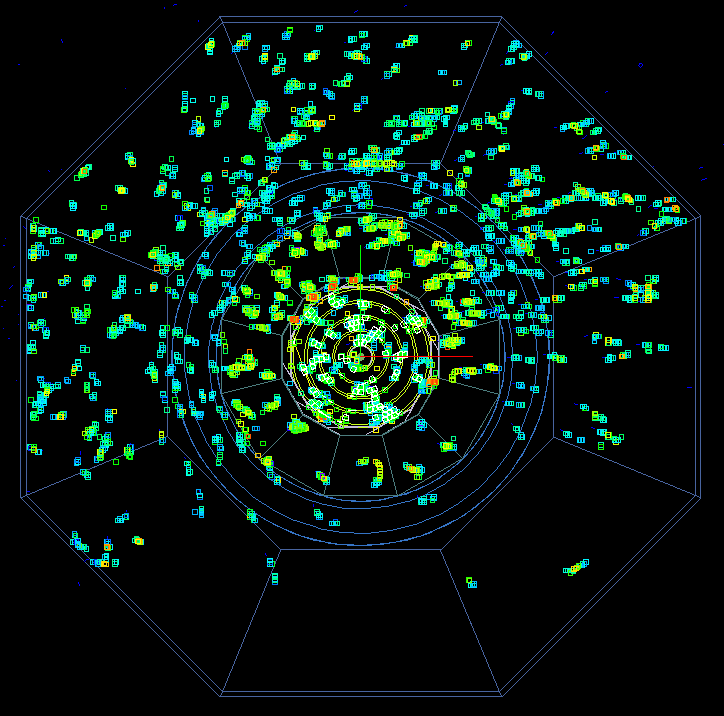
\includegraphics[width=\paperwidth]{muons_positron_5spoilers_wall_515_xyview_croped.png}}};
 % \tikz\node[opacity=0.2]{\centering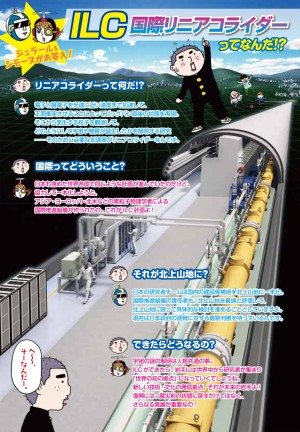
\includegraphics[height=\paperheight]{Iwatecomics.jpg}};
 }
\begin{frame}
  \titlepage
\end{frame}
}
\begin{frame}
  \tableofcontents
\end{frame}

\section{Muons from the muon spoilers}
\begin{frame}{The layout of the ILC}
\ilclogo
\begin{center}
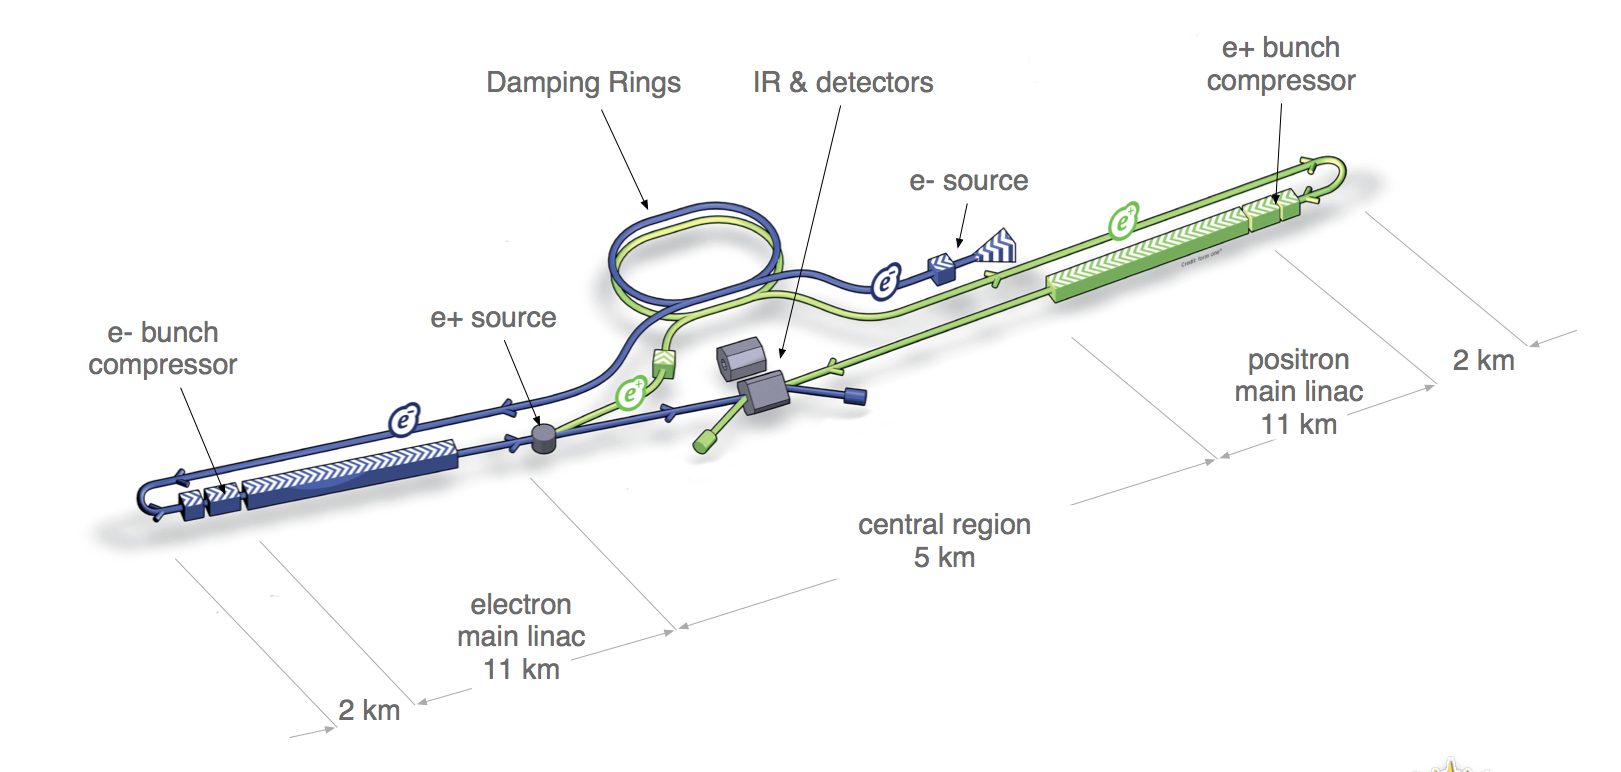
\includegraphics[width=\textwidth]{figures/ILC_schematic_layout.png}
\end{center}
The muon spoilers will be installed in the Beam Delivery System (BDS) in the central region.
\end{frame}

\begin{frame}{BDS tunnel layout}
\ilclogo
\begin{center}
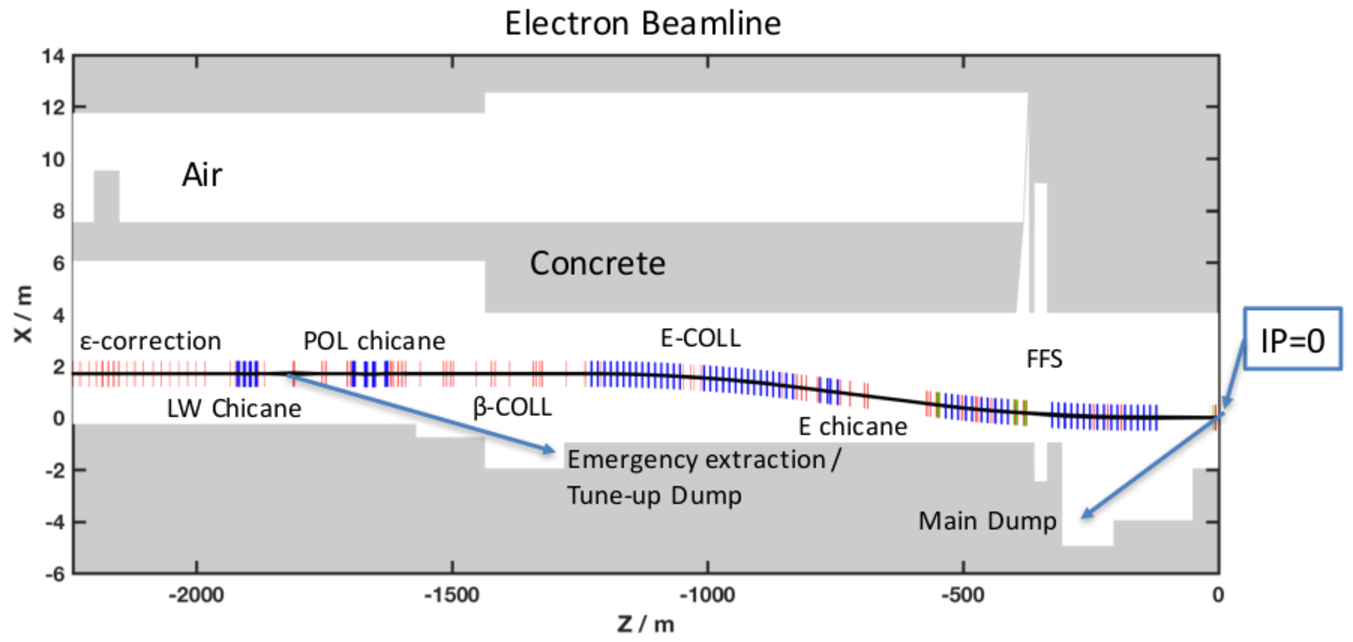
\includegraphics[height=0.65\textheight]{BDS_electron_tunnel.pdf}
\end{center}
\end{frame}

\subsection{Muon spoiler scenarios}
\begin{frame}{Muon spoiler scenarios}
\ilclogo
There are TWO SPOILER SCENARIOS under discussion:
\begin{itemize}
 \item \textbf{5 Spoilers}
 \item \textbf{5 Spoilers + Wall}
\end{itemize}

\begin{columns}[b]
 \begin{column}{0.8\textwidth}
 \flushright
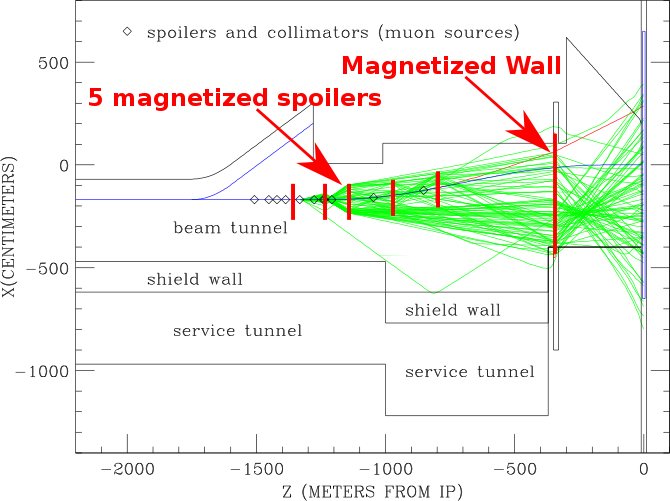
\includegraphics[height=0.67\textheight]{BDS_Tunnel_Spoilers+Wall.png}
\end{column}
 \begin{column}{0.2\textwidth}
 \flushleft
e\textsuperscript{-} beam line
\vspace*{0.55cm}
\end{column}
\end{columns}
\end{frame}

\begin{frame}{5 donut spoilers}
\ilclogo
\textbf{The donut spoilers} are designed as follows:
\begin{itemize}
 \item \unit[70]{cm} radius
 \item \unit[5]{m} long
 \item Magnetized iron with a field of $\sim$\unit[10-19]{kG}
 \item 5 locations (before IP):
 \begin{itemize}
  \item 802.5m
  \item 975.5m
  \item 1145.5m
  \item 1234.5m
  \item 1358.5m
 \end{itemize}

\end{itemize}
\begin{center}
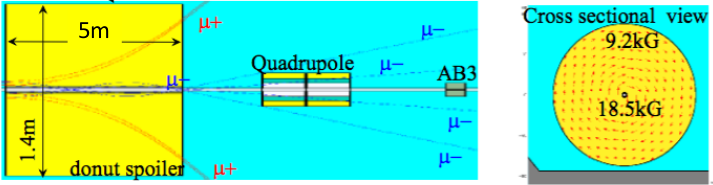
\includegraphics[height=0.3\textheight]{Spoiler.png}
\end{center}
\end{frame}

\begin{frame}{5 donut spoilers + wall}
\ilclogo
\textbf{The iron wall} would completely fill up the tunnel:
\begin{itemize}
 \item \unit[5]{m} x \unit[5]{m}, \unit[5]{m} long
 \item Magnetized with a field of $\sim$\unit[16]{kG}
 \item Located $\sim$\unit[400]{m} away from the IP
 \item Would cost $\sim$ \$3 million
\end{itemize}
\begin{center}
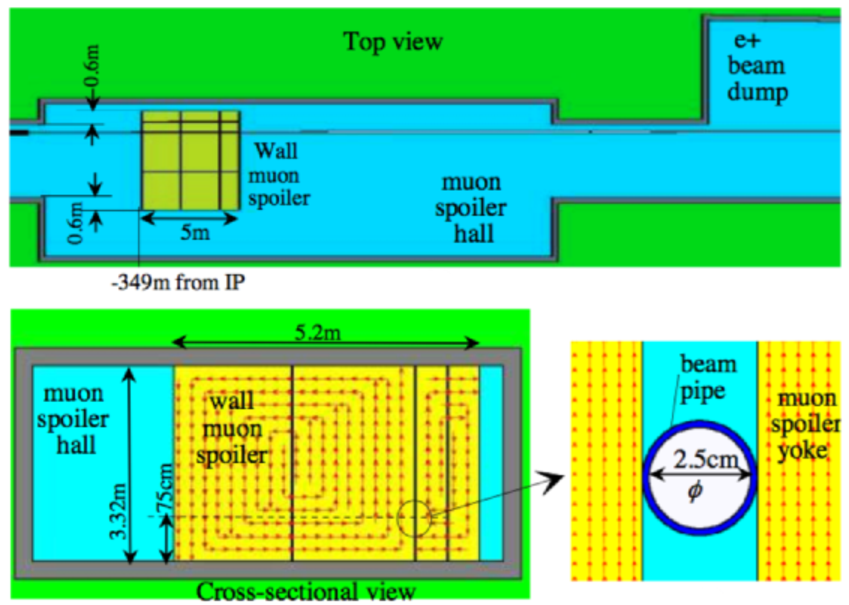
\includegraphics[height=0.7\textheight]{Muon_wall.pdf}
\end{center}
\end{frame}

\section{MUCARLO simulation}
\begin{frame}{MUCARLO simulation overview}
\ilclogo

\begin{columns}
 \begin{column}{0.7\textwidth}
  \begin{itemize}
\item BDS backgrounds with muon collimation system modelled with MUCARLO [Lewis Keller, SLAC] and Geant4 [Glen White, SLAC]
\item Using TDR baseline machine parameters for the ILC500
\item Muon production processes:
\begin{itemize}
\item Predominantly: Bethe-Heitler process:\\ \textgamma + Z $\rightarrow$ Z' + \textmu$^+$\textmu$^-$
\item Few \% level: direct annihilation of positrons with atomic electrons: e$^+$e$^-$ $\rightarrow$ \textmu$^+$\textmu$^-$
\end{itemize}
\item Halo particle tracking:
\begin{itemize}
\item Turtle with MUCARLO
\item Lucretia with a built-in Geant4 model interface
\end{itemize}
\end{itemize}

 \end{column}
 \begin{column}{0.3\textwidth}
  \includegraphics[width=\textwidth]{BetheHeitler.pdf}
 \end{column}
\end{columns}
\end{frame}

\subsection{Muon tracking}
\begin{frame}{Muon tracks in the BDS tunnel}
\ilclogo

\begin{columns}
 \begin{column}{0.3\textwidth}
  Muon tracks of positively (\textcolor{green}{\textmu\textsuperscript{+}}) and negatively (\textcolor{red}{\textmu\textsuperscript{-}}) charged muons, originating at a specific source location in the e\textsuperscript{-} beam line:
 \end{column}
 \begin{column}{0.65\textwidth}
  \begin{center}
\includegraphics[width=\textwidth]{e-_beam_traj_hor.pdf}
\end{center}
 \end{column}
\end{columns}

\small The tracks that are drawn are only the ones that reach the detector.\\
\small The spoiler polarities are set to defocus muons with the same charge as the beam charge. $\rightarrow$ More \textmu\textsuperscript{+} from the e\textsuperscript{-} beam than from the e\textsuperscript{+} beam, and vice versa.
\end{frame}

\subsection{Muon 4-vectors}
\begin{frame}{Muons in the detector}
\ilclogo
4-vectors of the muons are given to SiD and ILD for studying the effect of the muons on the detector performance.\\
\vspace*{0.2cm}
\begin{tabular}{ll}
\textbf{Scenario} & \textbf{Number of muons in a detector with 6.5m radius}\\
 5 Spoilers& 4.3 muons/bunch crossing\\
 5 Spoilers + Wall & 0.6 muons/bunch crossing
\end{tabular}
\end{frame}

\section{Motivation}
\begin{frame}{}
\ilclogo
Question to SiD and ILD: Do we need the muon wall at all?!
MID people would be happy to get rid of it because of safety issues, and the costs for such a iron wall.
\begin{center}
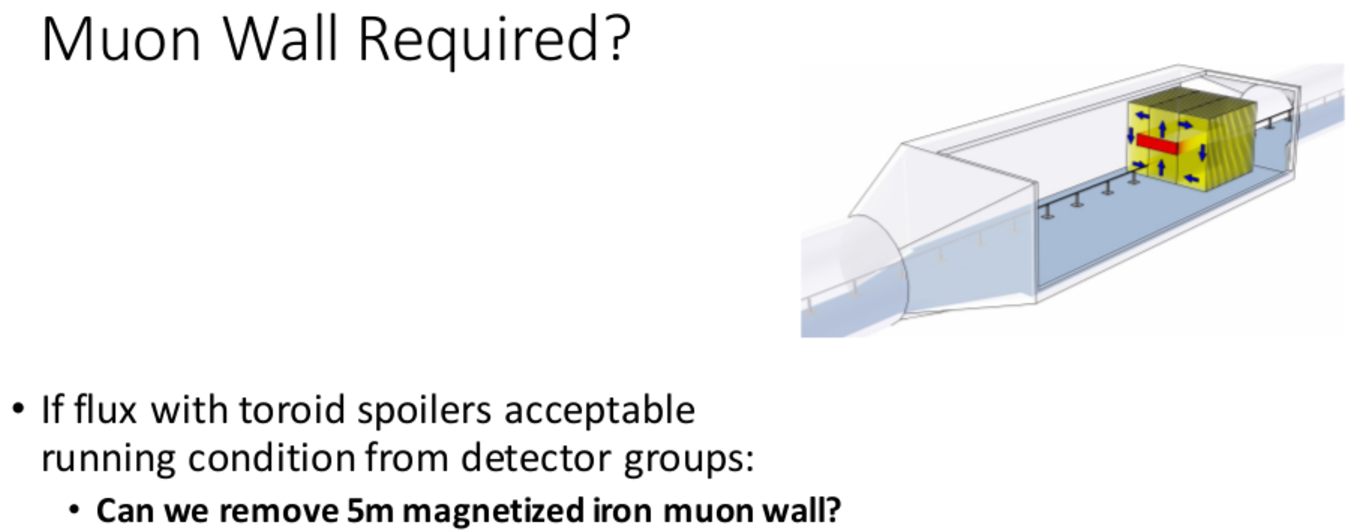
\includegraphics[height=0.5\textheight]{Muon_wall_required.pdf}
\end{center}
\end{frame}

\section{Results}
\begin{frame}{Analysis Method}
\ilclogo
Analysis method:
\begin{itemize}
\item 4-vector files provided by Lewis Keller:
\begin{itemize}
 \item 5 Spoilers + Wall: from electron line: $\sim$4321 muons
 \item 5 Spoilers + Wall: from positron line: $\sim$5834 muons
 \item 5 Spoilers: from electron line: $\sim$30292 muons
 \item 5 Spoilers: from positron line: $\sim$33482 muons
\end{itemize}
\item Conversion of the text files with the 4-vector values to  STDHEP files.
\item The STDHEP files were used as input to a full SiD detector simulation with Geant4.
\item Nice event displays from the simulations with WIRED4 in JAS3.
\item Studies of the spatial distributions, the muon energy, the timing, and the detector occupancies.
\end{itemize}

\end{frame}

\subsection{Event displays of muons in the SiD detector}
\begin{frame}{WIRED4 event display - 5 Spoilers + Wall}
\sidlogo
1 train's worth of muons ($\sim$ 515 muons) \textbf{from the positron line only}:
\begin{center}
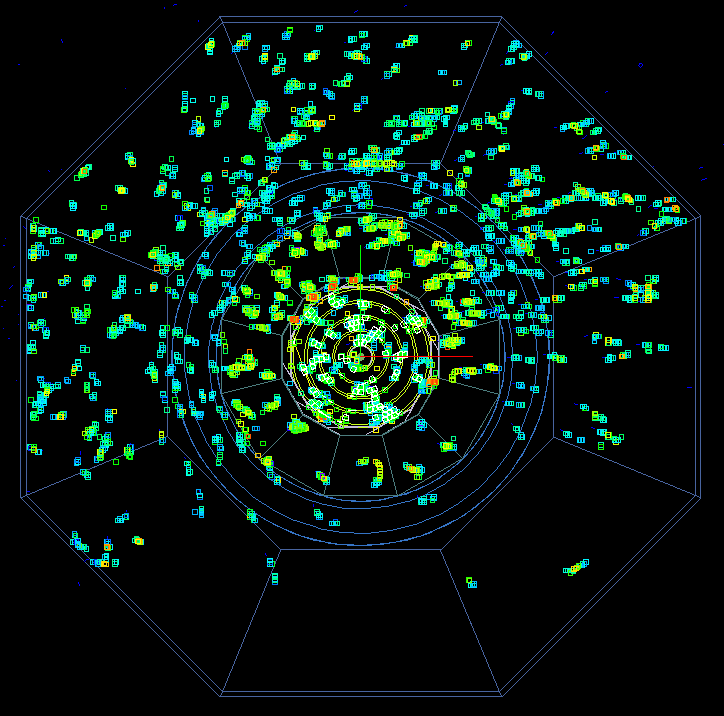
\includegraphics[height=0.6\textheight]{muons_positron_5spoilers_wall_515_xyview_croped.png}
{\tiny xy-view}
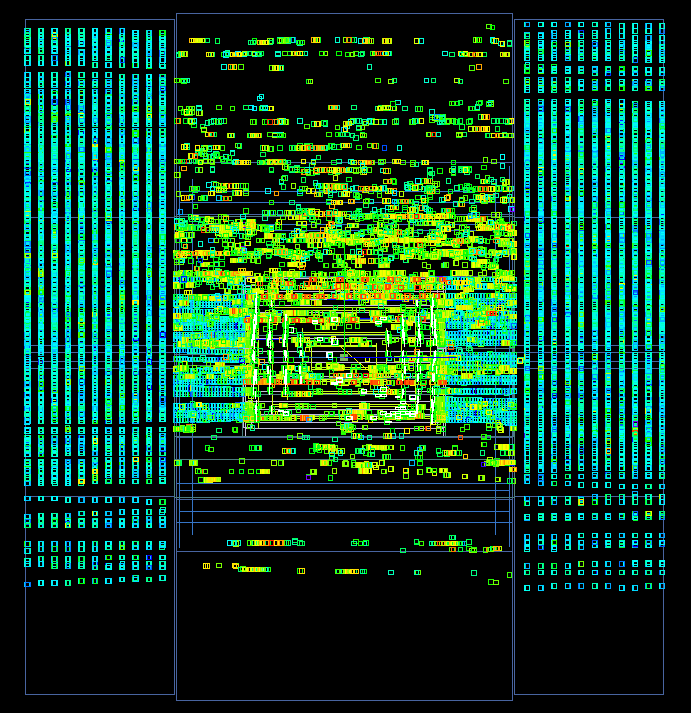
\includegraphics[height=0.6\textheight]{muons_positron_5spoilers_wall_515_zyview_croped.png}
{\tiny zy-view}
\end{center}
Together with the muons from the e\textsuperscript{-} line, there will be \textbf{$\sim$ 900 muons per train in the '5 Spoilers + Wall' scenario}.
\end{frame}
\begin{frame}{WIRED4 event display - 5 Spoilers}
\sidlogo
1 train's worth of muons ($\sim$ 2961 muons) \textbf{from the positron line only}:
\begin{center}
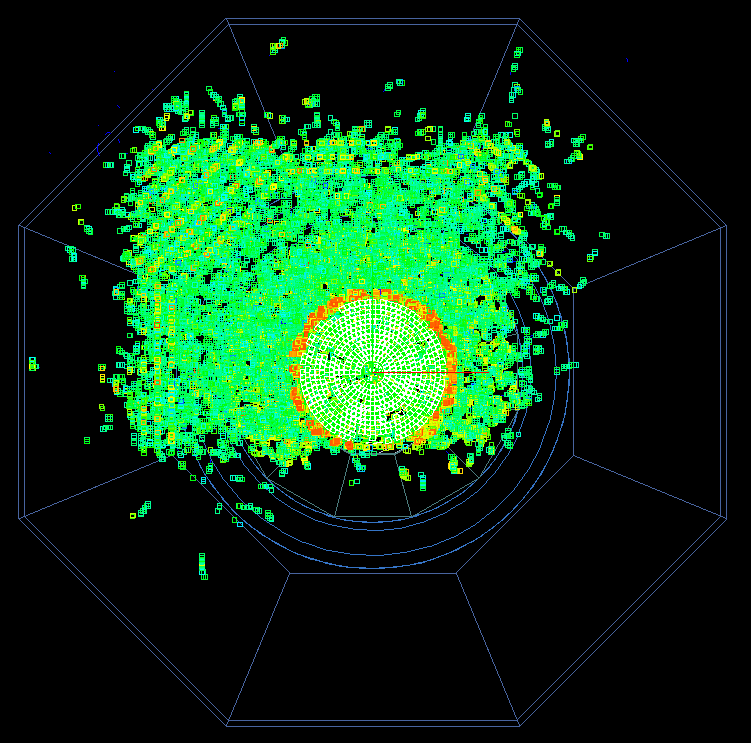
\includegraphics[height=0.6\textheight]{muons_positron_5spoilers_2961_xyview_croped.png}
{\tiny xy-view}
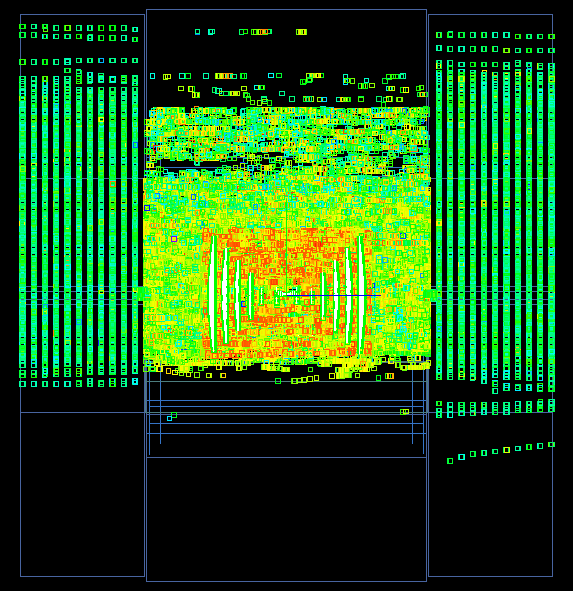
\includegraphics[height=0.6\textheight]{muons_positron_5spoilers_2961_zyview_croped.png}
{\tiny zy-view}
\end{center}
Together with the muons from the e\textsuperscript{-} line, there will be \textbf{$\sim$ 5600 muons per train in the '5 Spoilers' scenario}.\\
The spatial distribution is due to the tunnel shape and its shielding effects.
\end{frame}

%New command: column type
\newcolumntype{P}[1]{>{\centering}p{#1}}

\subsection{Analysis - Spatial distributions}
\begin{frame}{Explanation of spatial distributions}
\sidlogo
 \begin{center}
\includegraphics[height=0.85\textheight]{Explanation_Spatial_distribution_NEW.pdf}
\end{center}
\end{frame}

\subsection{Analysis - Energy distributions}
\begin{frame}{Energy distribution of muons}
\sidlogo
\begin{columns}
 \begin{column}{0.25\textwidth}
 \small
  Comparison of the muon energies in the \textcolor{red}{'5 Spoilers'} and the \textcolor{blue}{'5 Spoilers + Wall'} case:
 \end{column}
 \begin{column}{0.75\textwidth}
  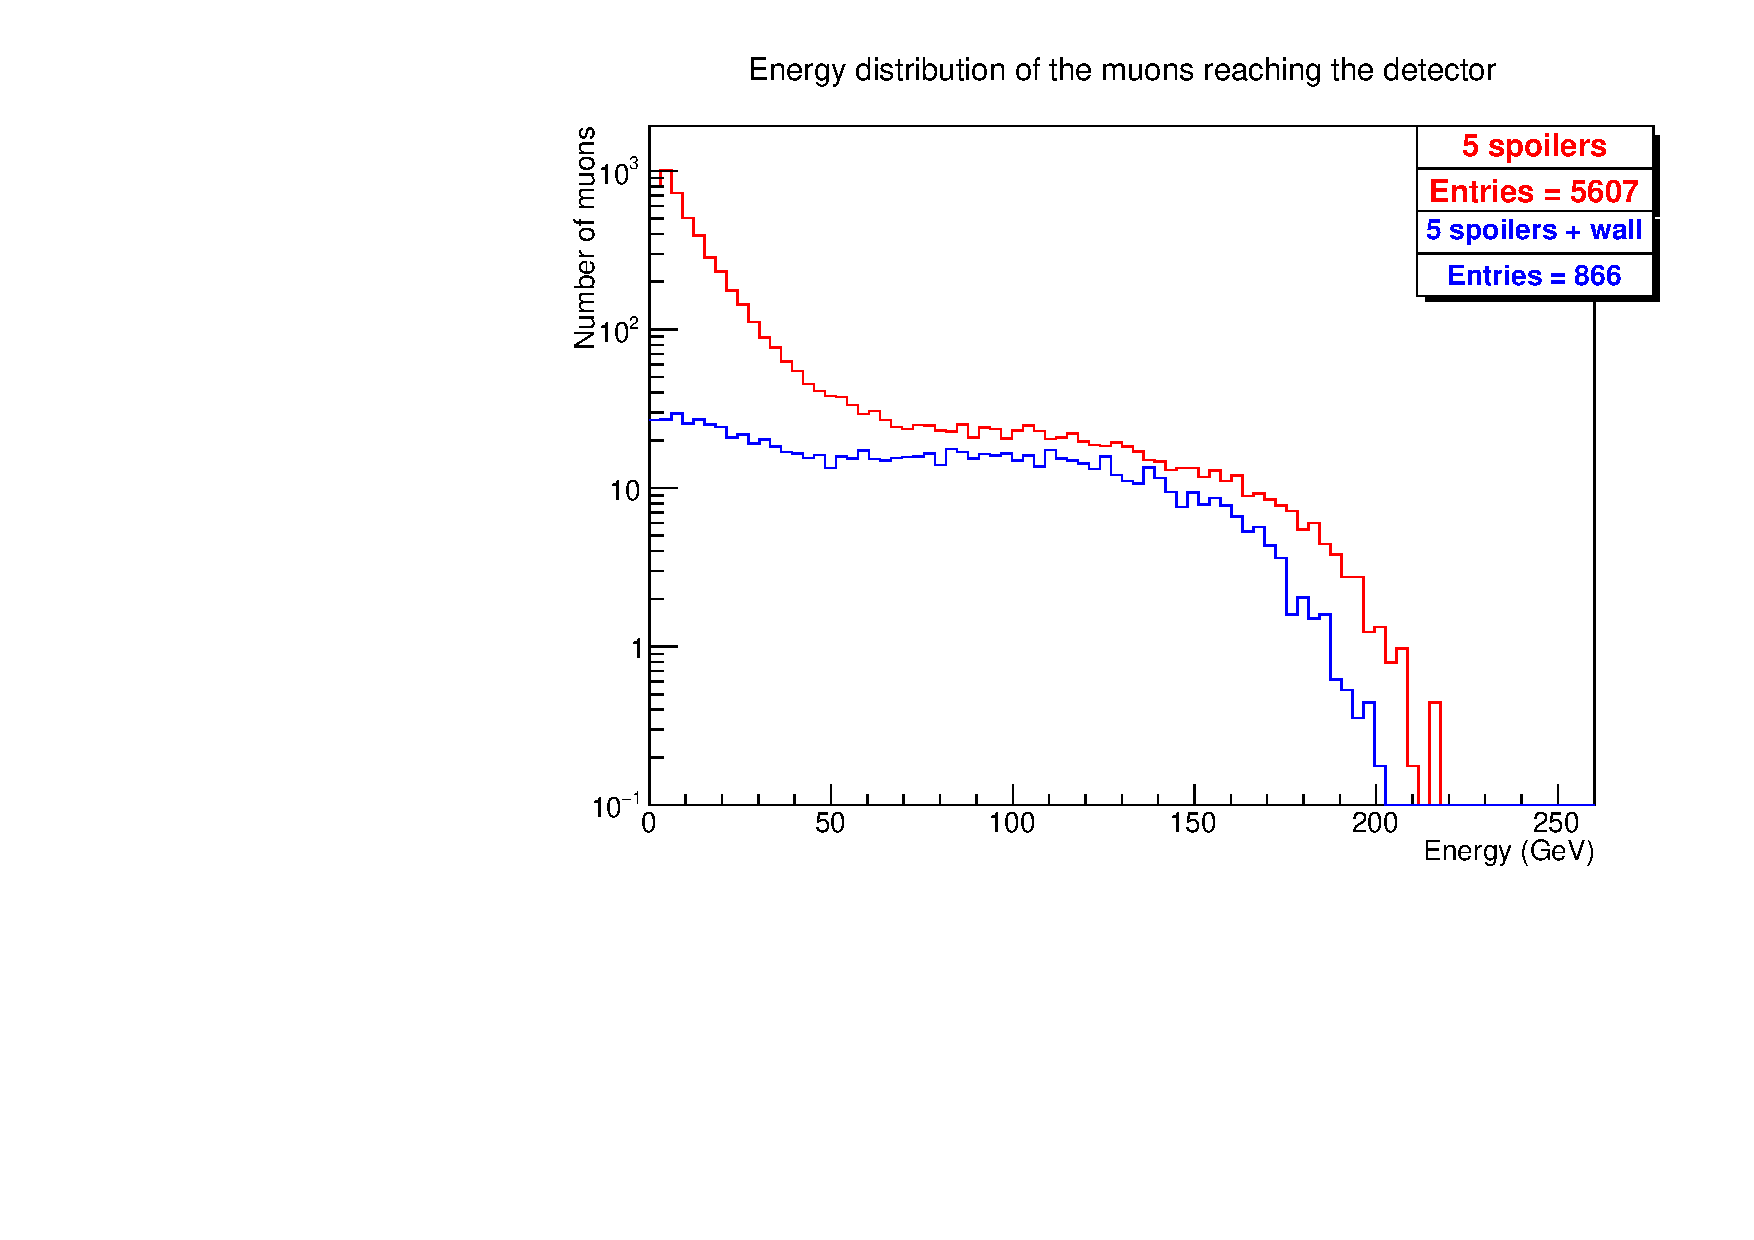
\includegraphics[width=\textwidth]{figures/muon_energy.pdf}
 \end{column}
\end{columns}
In the 'Spoiler + Wall' case, the lower energy muons are either stopped or deflected by the magnetized wall.
\end{frame}

\subsection{Analysis - Total number of hits}
\begin{frame}{Total number of hits}
\sidlogo
\begin{columns}
 \begin{column}{0.23\textwidth}
 \small
  Comparison of the total number of hits in the different SiD subdetectors in the \textcolor{red}{'5 Spoilers'} and the \textcolor{blue}{'5 Spoilers + Wall'} case:
 \end{column}
 \begin{column}{0.8\textwidth}
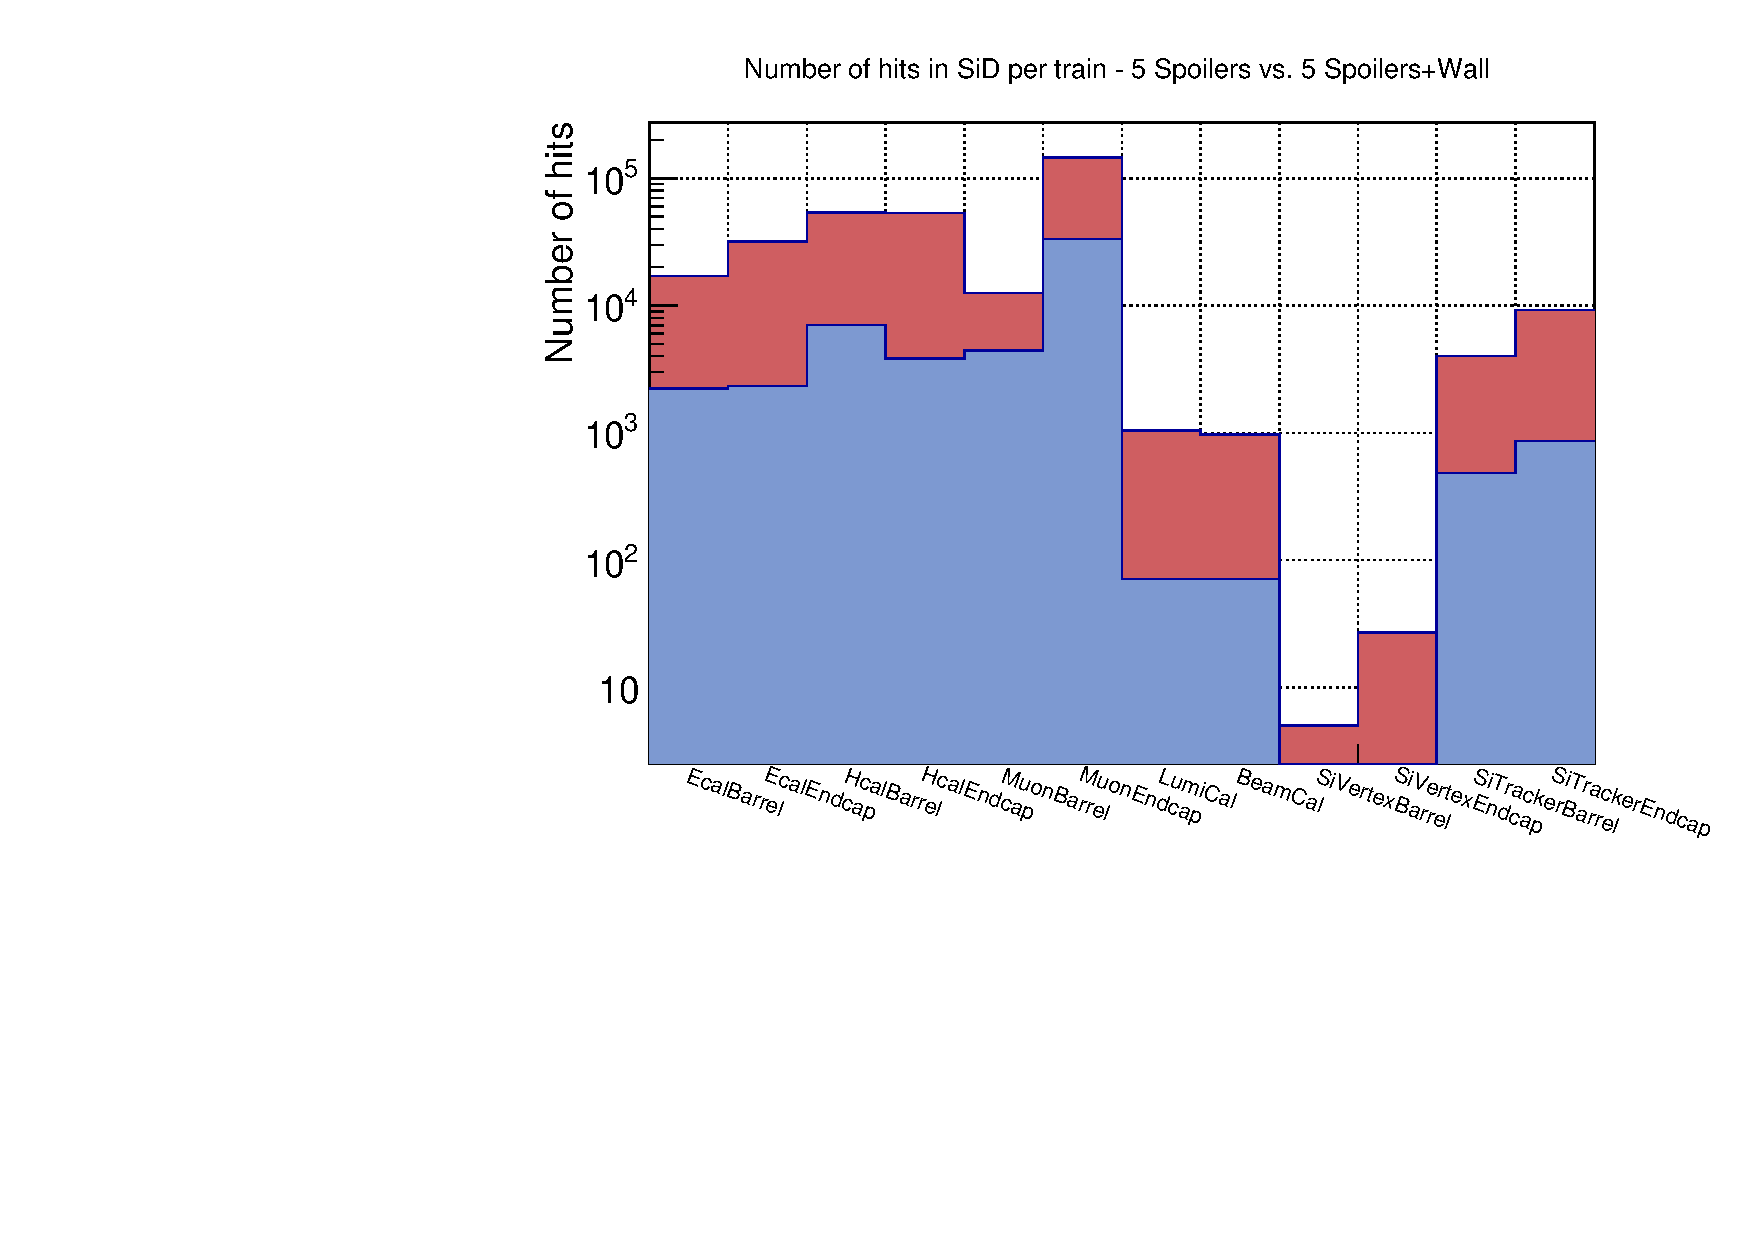
\includegraphics[width=\textwidth]{figures/Hits_in_SiD_subdetectors_MuonSpoilerStudy.pdf}
 \end{column}
\end{columns}
\begin{center}
\begin{tabular}{@{}p{0.343\textwidth}p{0.01\textwidth}p{0.18\textwidth}p{0.01\textwidth}p{0.343\textwidth}p{0.001\textwidth}@{}}
 \centering Vertex detectors & < & \centering ECAL, HCAL & < & \centering MuonEndcaps & \\
  \centering{\scriptsize Smallest effective detector area} & &  \centering{\scriptsize Particle showers} & &  \centering{\scriptsize Biggest effective detector area}&
\end{tabular}
\end{center}
\end{frame}

\begin{frame}{Explanation of hit number distribution -\\ \small Spatial distribution in the MuonEndcaps}
\sidlogo
 \begin{center}
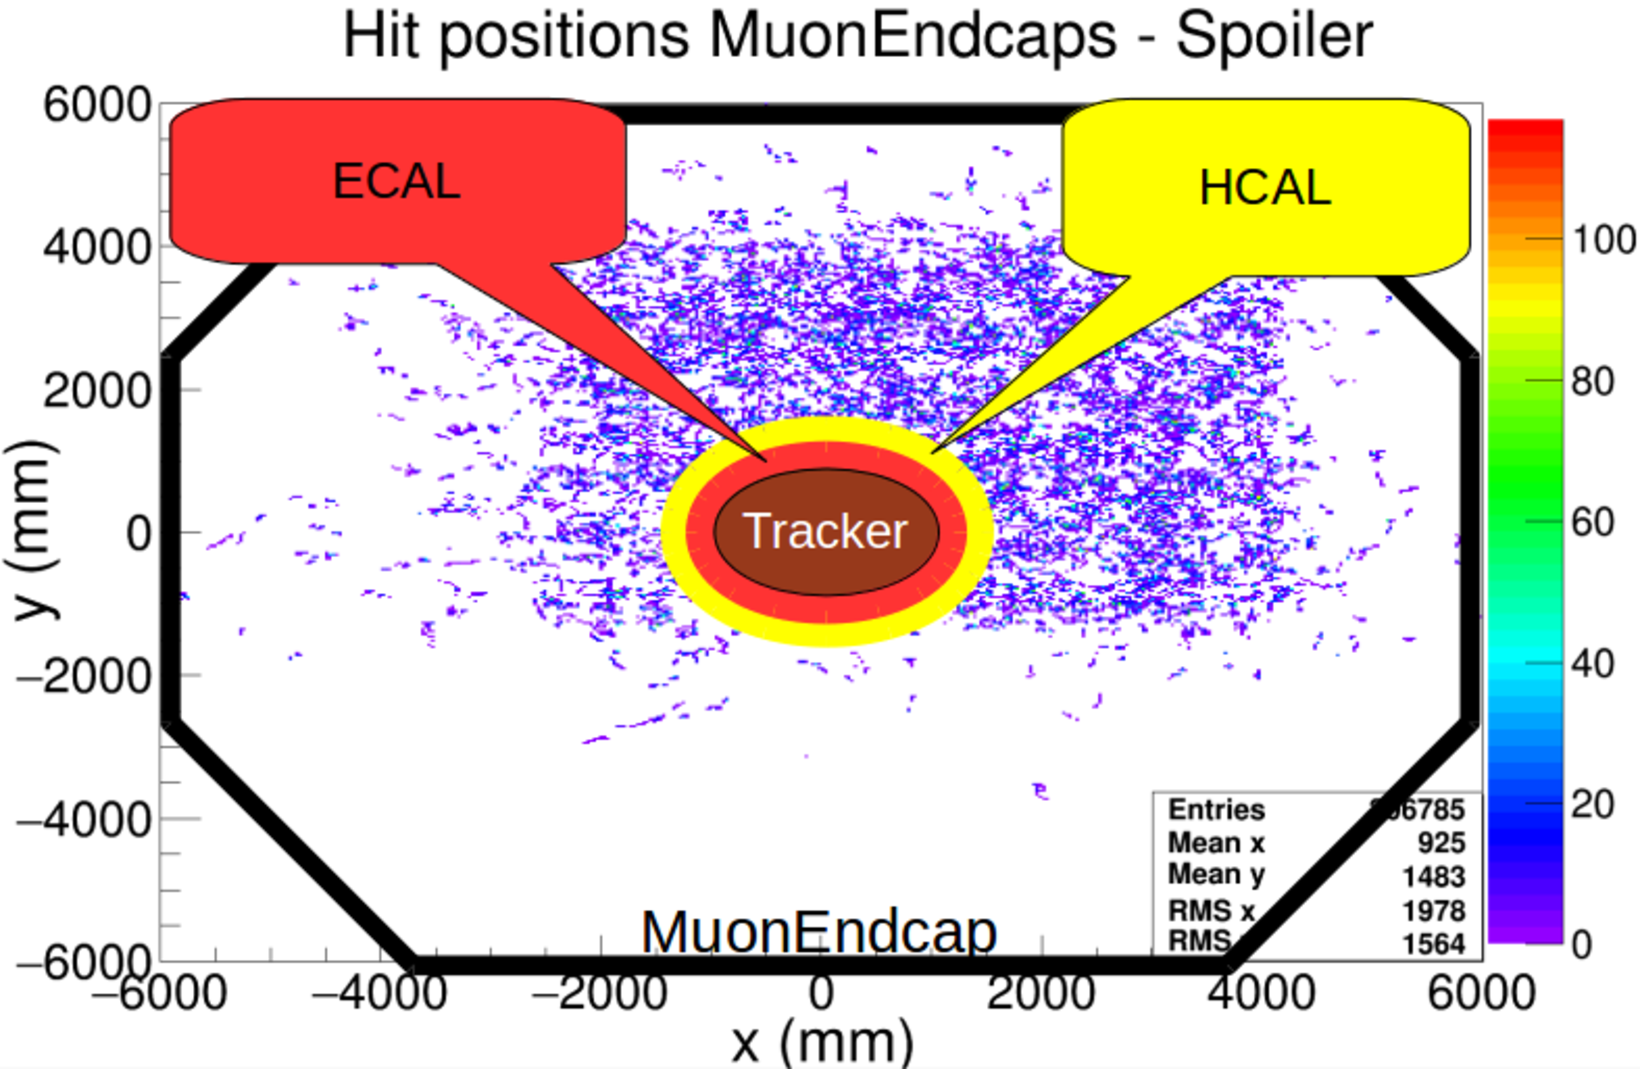
\includegraphics[height=0.78\textheight]{Explanation_Hits_Subdetectors.pdf}
\end{center}
\end{frame}

\subsection{Analysis - Occupancies}
\begin{frame}{Occupancy plots - \small SiTrackerEndcap}
\sidlogo
\begin{columns}
 \begin{column}{0.25\textwidth}
 \small
  Comparison of the muon occupancy in the \textcolor{red}{'5 Spoilers} and the \textcolor{blue}{'5 Spoilers + Wall'} case.\\{\small The \textcolor{green}{buffer depth} of the current sensor design is 4.}\\
  \vspace*{0.2cm}
  {\footnotesize The following occupancy plots are normalized by the first bin.}
 \end{column}
 \begin{column}{0.75\textwidth}
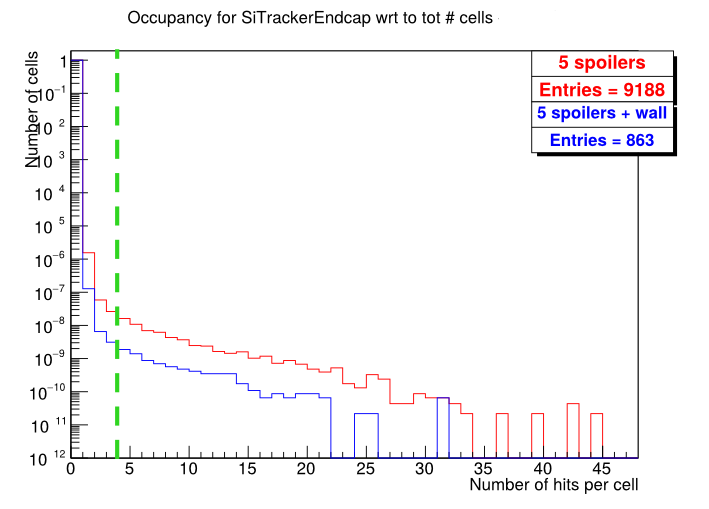
\includegraphics[width=\textwidth]{figures/SiTrackerEndcap_Occupancy.png}
\end{column}
\end{columns}
For both scenarios, 5 Spoilers w/ and w/o Wall, 10$^{-9}$ - 10$^{-7}$ of all cells that get hit have 4 hits.
\end{frame}
\begin{frame}{Occupancy plots - \small EcalEndcap}
\sidlogo
 \begin{center}
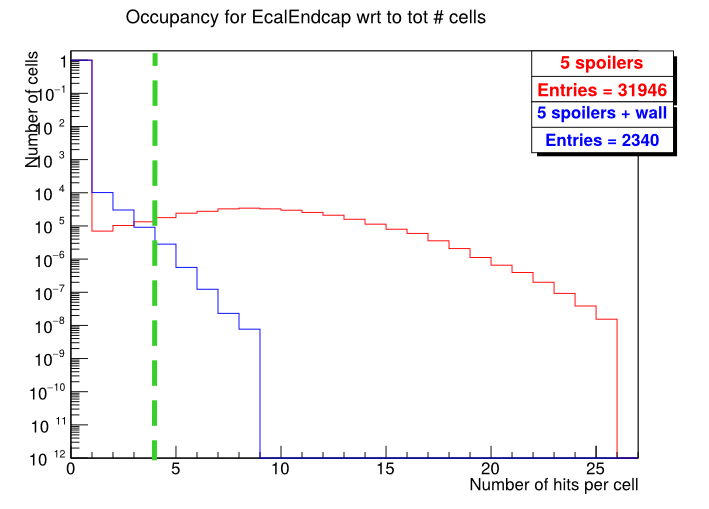
\includegraphics[height=0.62\textheight]{figures/EcalEndcap_Occupancy.png}
\end{center}
\small '5 Spoilers + Wall' seems to do better by an order of magnitude, when looking at a buffer depth of 4. The occupancy is still at a level of only $\sim$10$^{-6}$.\\
\small The '5 Spoiler' case shows up to 27 hits per cell.$\rightarrow$ Constant occupancy for all buffer depths.
\end{frame}

\subsection{Analysis - Dead cells}
\begin{frame}{Dead cells - \small SiTrackerEndcap}
\sidlogo
 \begin{center}
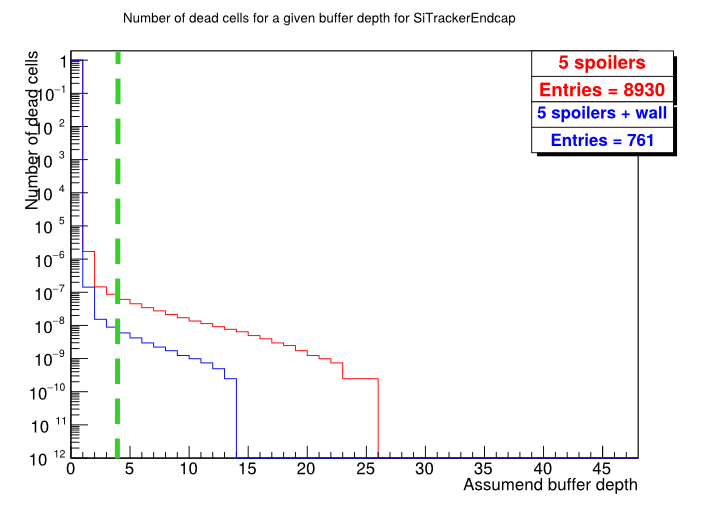
\includegraphics[height=0.65\textheight]{figures/SiTrackerEndcap_DeadCells.png}
\end{center}
\small For an assumed buffer depth of 4, the total number of dead cells is different by an order of magnitude. $\rightarrow$ In the '5 Spoiler' case, 10$^{-7}$ cells would have reached the buffer limit.
\end{frame}
\begin{frame}{Dead cells - \small EcalEndcap}
\sidlogo
 \begin{center}
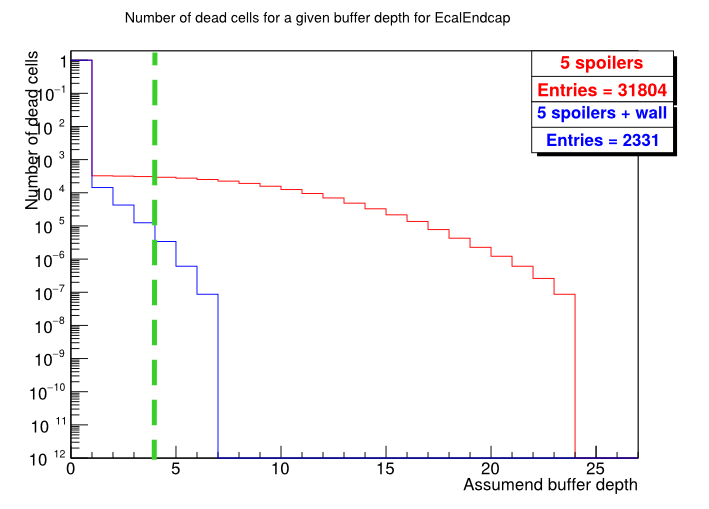
\includegraphics[height=0.65\textheight]{figures/EcalEndcap_DeadCells.png}
\end{center}
\small For an assumed buffer depth of 4, the total number of dead cells is different by about two orders of magnitude. $\rightarrow$ In the '5 Spoiler' case, 10$^{-3}$ cells would have reached the buffer limit.
\end{frame}

\subsection{Analysis - Time distributions}
\begin{frame}{Creation time distribution}
\sidlogo
All of the primary muons are created up to 0.5\,ns after the bunch passing the material.
 \begin{center}
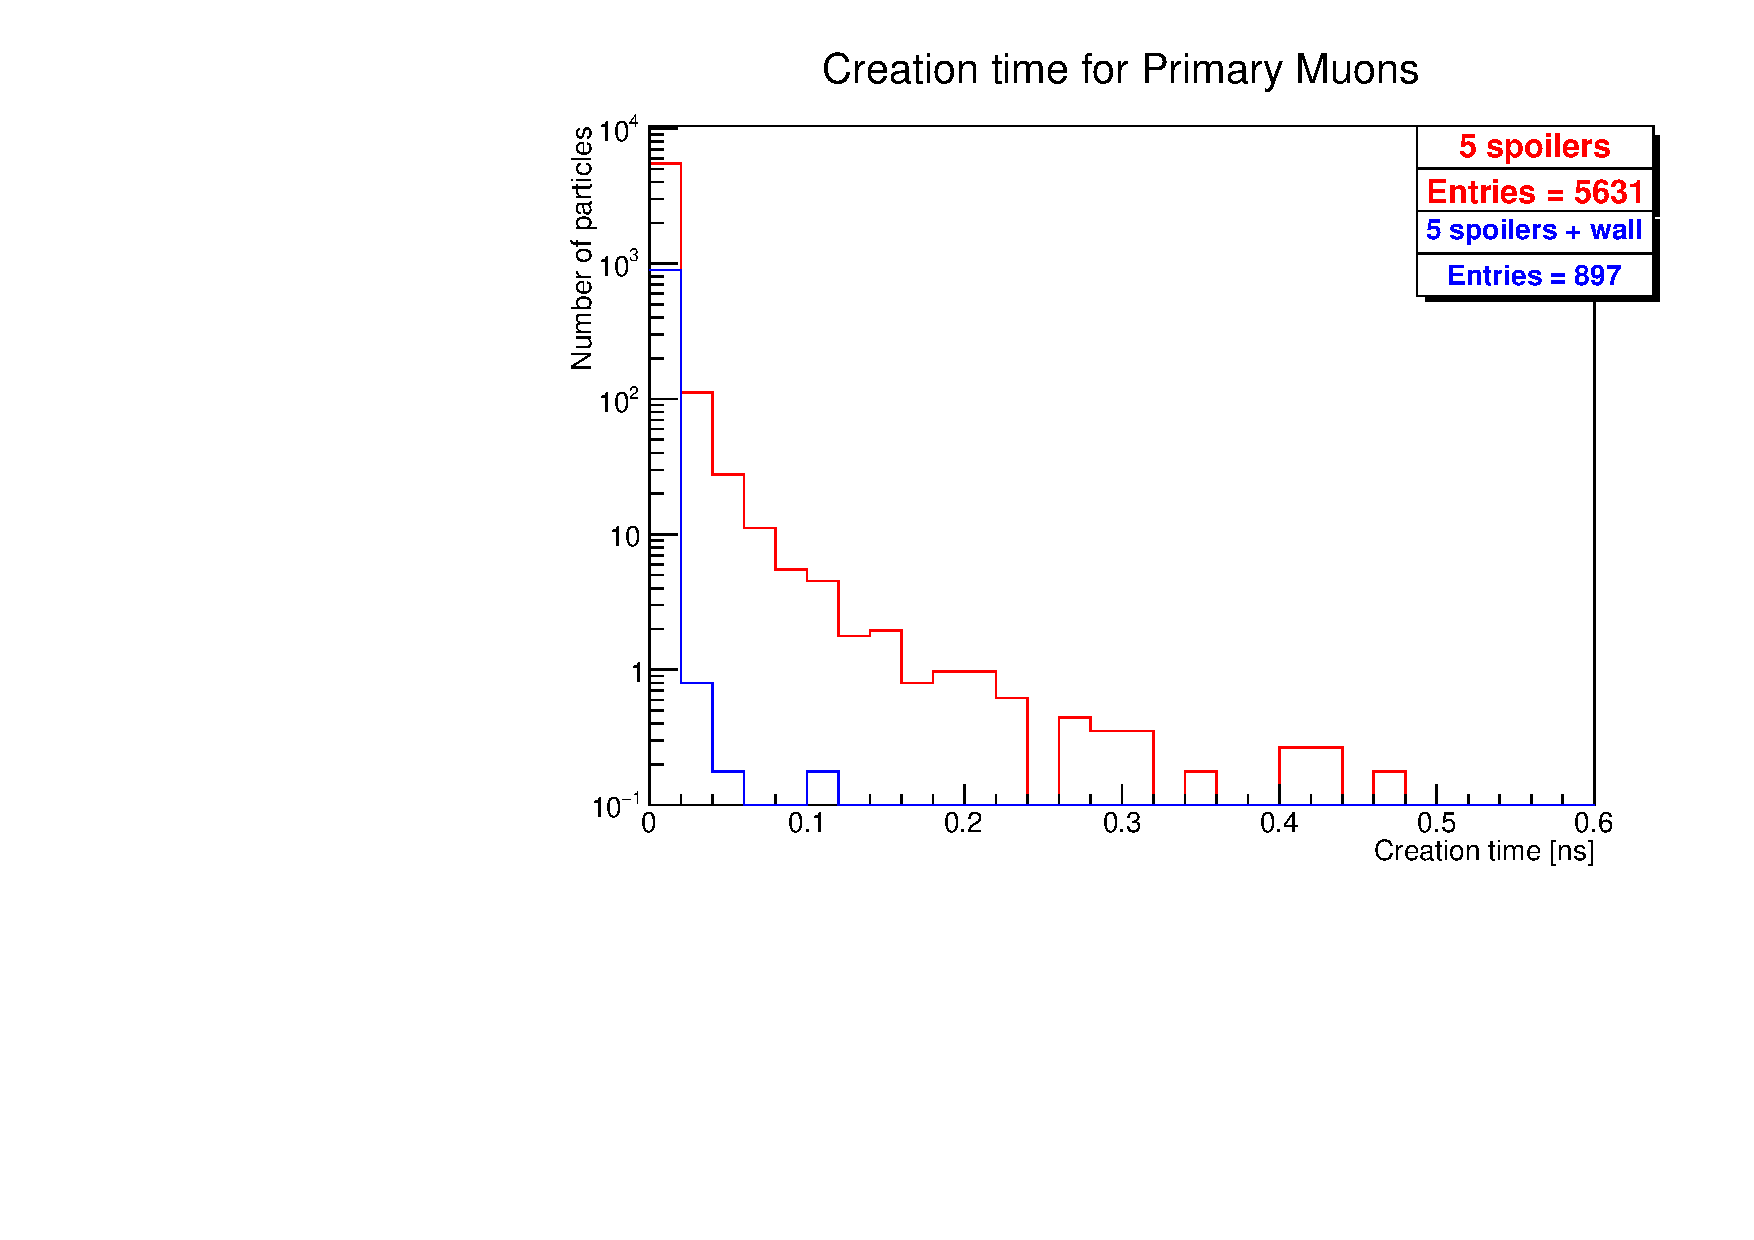
\includegraphics[height=0.65\textheight]{figures/muon_creationtime.pdf}
\end{center}
The lower energy muons, which have a broader creation time, do not reach the detector in the '5 Spoilers + Wall' case.
\end{frame}
\begin{frame}{Hit Time distribution - \small MuonEndcaps}
\sidlogo
 \begin{center}
\includegraphics[height=0.65\textheight]{figures/muon_hittime_all_layers_MuonEndcap.pdf}
\end{center}
Muons are first hitting the MuonEndcaps as the most outer subdetector.
\end{frame}
\begin{frame}{Hit Time distribution - \small EcalEndcaps}
\sidlogo
Hit time distributions for \\
\hspace*{0.6cm} the PRIMARY MUONS and the SHOWER PARTICLES:
 \begin{center}
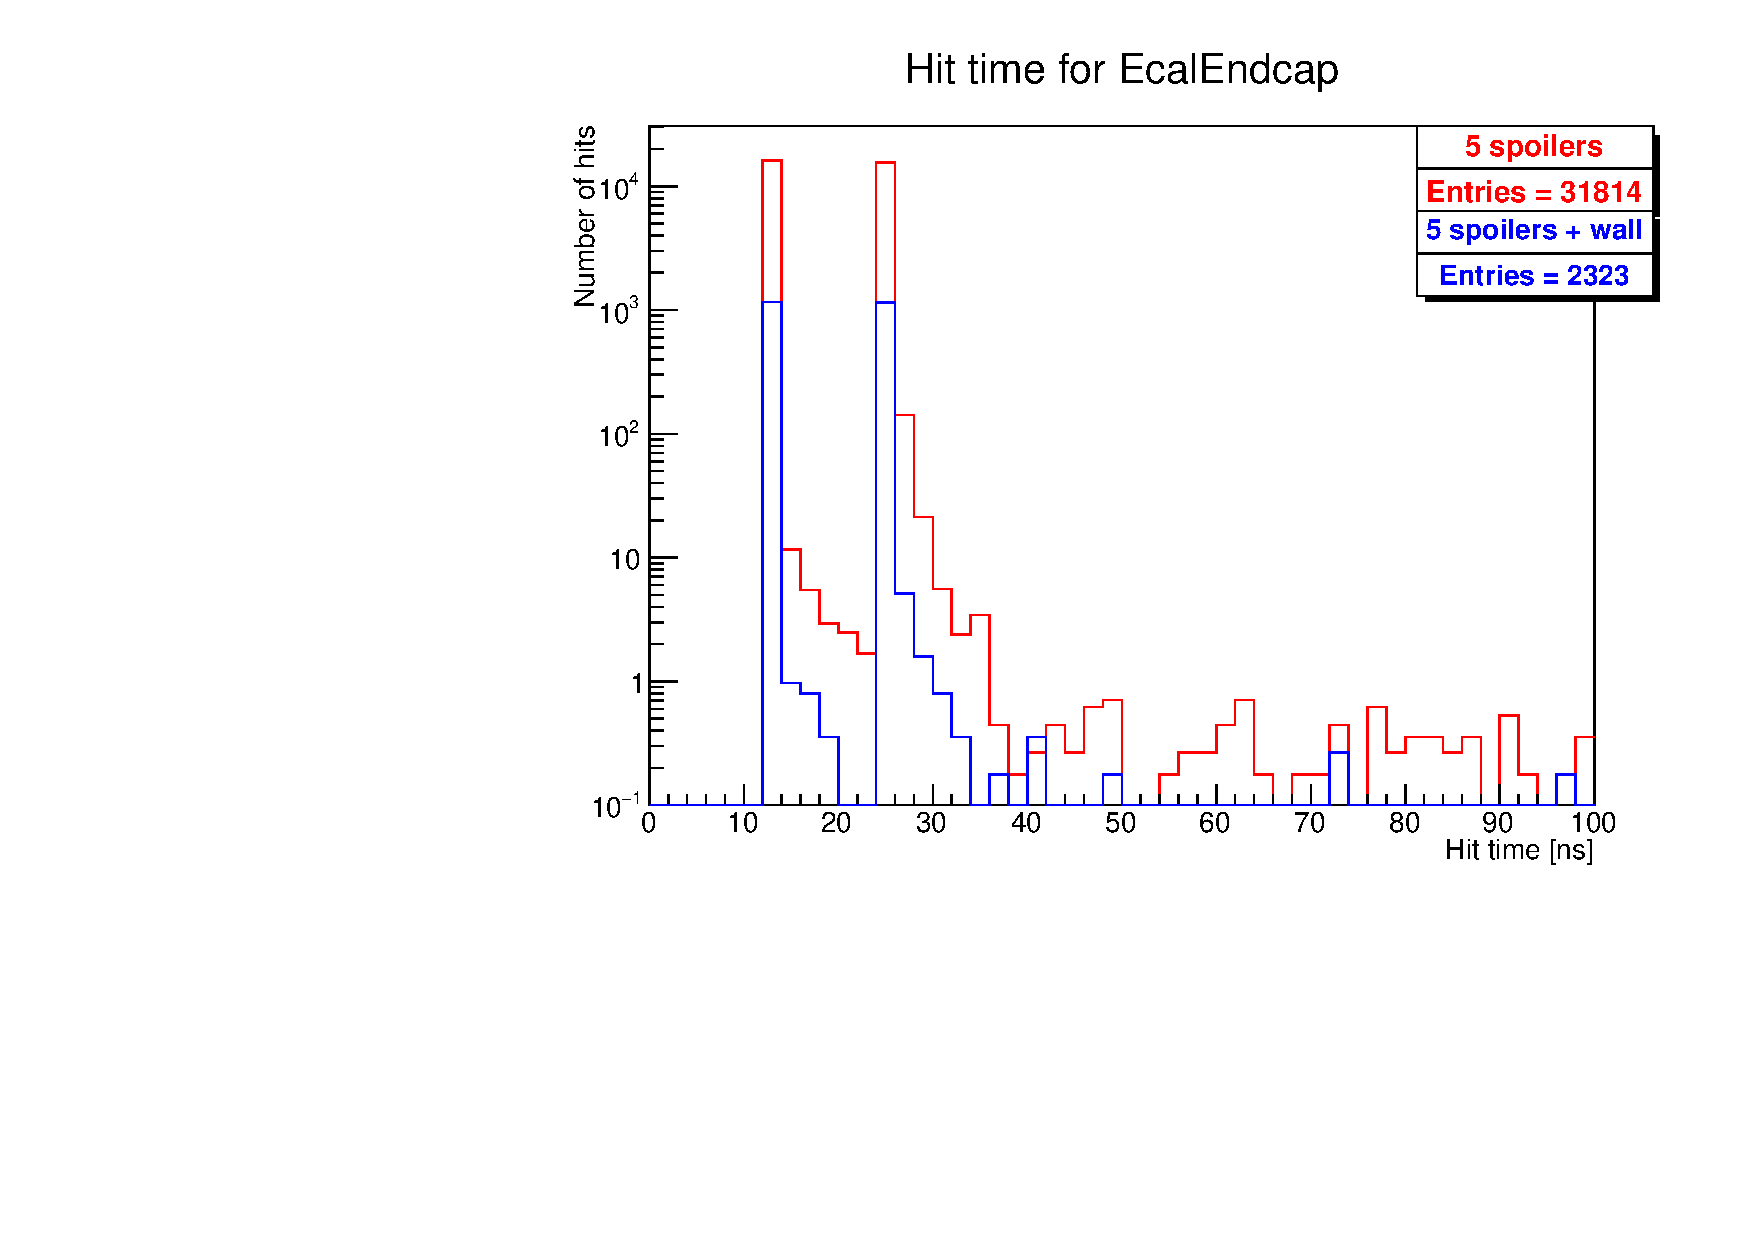
\includegraphics[height=0.5\textheight]{figures/muon_hittime_all_layers_EcalEndcap.pdf}
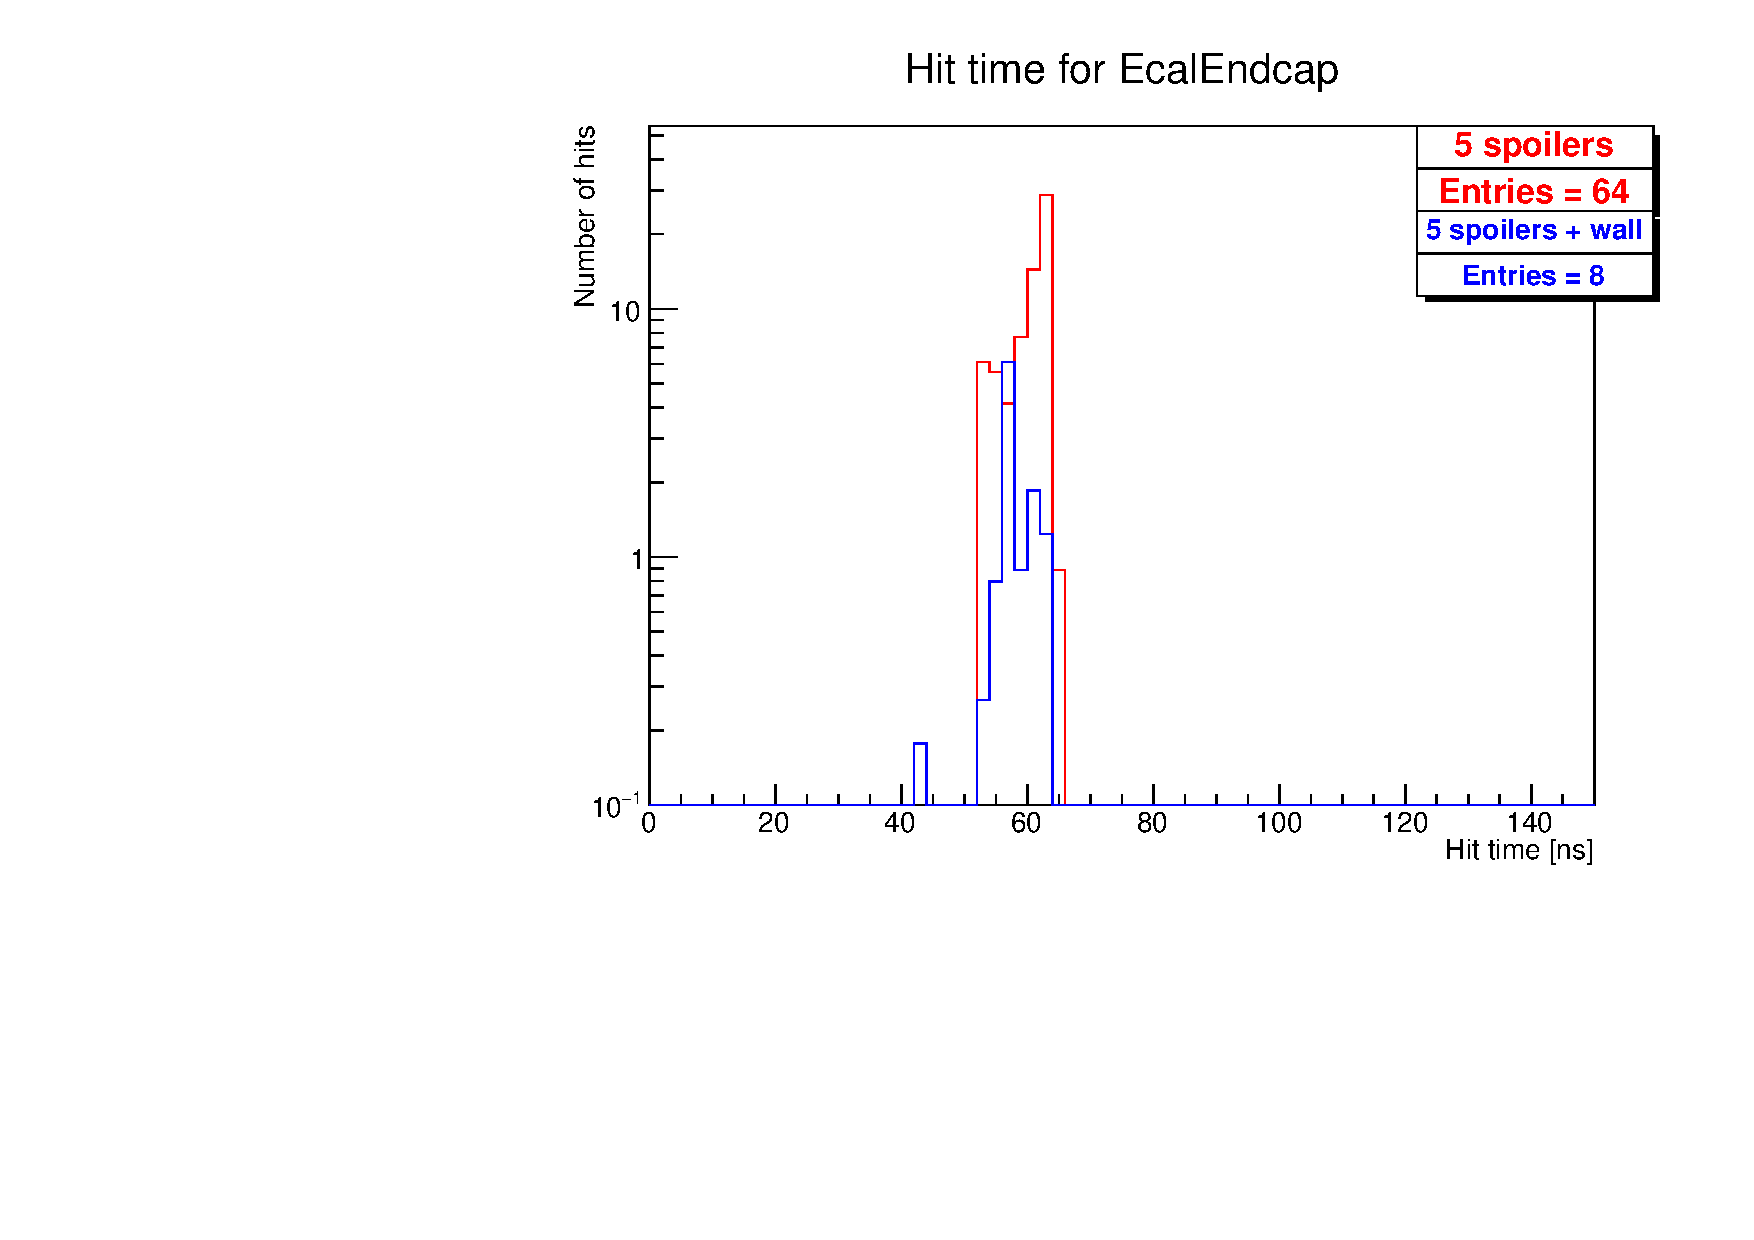
\includegraphics[height=0.5\textheight]{figures/muon_hittime_all_layers_shower_EcalEndcap.pdf}
\end{center}
The primary muons leave hits between 12 and $\sim$ 50\,ns after the bunch crossing, whereas the shower particles hit the EcalEndcaps about 60\,ns after the crossing.
\end{frame}
\begin{frame}{Hit Time distribution - \small SiTrackerEndcaps}
\sidlogo
Hit time distributions for \\
\hspace*{0.6cm} the PRIMARY MUONS and the SHOWER PARTICLES:
 \begin{center}
\includegraphics[height=0.5\textheight]{figures/muon_hittime_all_layers_SiTrackerEndcap.pdf}
\includegraphics[height=0.5\textheight]{figures/muon_hittime_all_layers_shower_SiTrackerEndcap.pdf}
\end{center}
The primary muons leave hits between 12 and $\sim$ 40\,ns after the bunch crossing, whereas the shower particles hit the Tracker endcaps about 40-100\,ns after the crossing.
\end{frame}

\subsection{Analysis - Shower particles}
\begin{frame}{PDG IDs of the shower particles}
\sidlogo
Shower particles created from muons in 1 train:
 \begin{center}
\includegraphics[height=0.65\textheight]{figures/Shower_PDGs.png}
\end{center}
Mainly electrons, positrons and photons.
\end{frame}

\section{Conclusion and Outlook}
\begin{frame}
\textit{Conclusion:}
\begin{itemize}
\item Low energy muons are stopped/deflected by the magnetized wall.
\item High energy muons could be used for tracker alignment.
\item Spatial distributions quite different in the '5 Spoiler' and '5 Spoiler+Wall' scenarios.
\item Number of hits in subdetectors are explained by different geometries.
\item Primary muons are instantaneous in comparison to e.g. pair background, but hits (also from shower particles) still up to $\sim$ 100\,ns after bunch crossing.
\item \textbf{\alert{Occupancy is small, but SiD would prefer:}}
\end{itemize}
\end{frame}
\begin{frame}
\textit{Outlook:}
\begin{columns}
 \begin{column}{0.65\textwidth}
  \begin{itemize}
\item \textbf{PACMAN} should be included in the SiD geometry.
This will have a big effect on the backgrounds, not only the muon spoiler background $\rightarrow$ PACMAN will stop muons with energies below 3-4 GeV.
\item Muon background will be used for \textbf{further Occupancy studies together with different other background sources}.\\
\small Detailed occupancy studies with different background sources (e.g. pair background) is being done for SiD. $\rightarrow$ SiD background note: ``A Study of the Impact of High Cross Section ILC Processes on the SiD Detector Design''\\( http://arxiv.org/abs/1609.07816 )
\end{itemize}
 \end{column}
 \begin{column}{0.35\textwidth}
  \includegraphics[height=0.37\textheight]{SiDPacman.jpg}
 \end{column}
\end{columns}
\vspace*{0.2cm}
\alert{
$\rightarrow$\textit{Stay tuned!}}
\end{frame}

\section{References}
\begin{frame}{References}
\tiny
\begin{thebibliography}{9}
\setbeamertemplate{bibliography item}[text]
\bibitem{MUCARLO_talk}  \emph{ECFA 2016: Talk by Glen White about the MUCARLO simulation of the muons from the muon spoilers}. \url{https://agenda.linearcollider.org/event/7014/contributions/34689/attachments/30076/44961/ILC_muons.pptx}
\bibitem{Jonas_talk}  \emph{DESY summer student program: Talk by Jonas Glomitza (RWTH Aachen) about ``The Impacts of the Muon Spoiler Background on the ILC Detector Performance'', 08. September 2016}. \url{https://indico.desy.de/getFile.py/access?contribId=9&resId=0&materialId=slides&confId=15972}
\bibitem{Suppression}  \emph{FERMILAB-CONF-07-276-AD: ``Suppression of Muon Backgrounds generated in the ILC Beam Delivery System'', Drozhdin et.al, 2007}. \url{https://inspirehep.net/record/771808/files/fermilab-conf-07-276.pdf}
\bibitem{MUCARLO}  \emph{``Calculation of Muon Background in Electron Accelerators using the Monte Carlo Computer Program MUCARLO'', Rokni et.al}. \url{http://www.slac.stanford.edu/cgi-wrap/getdoc/slac-pub-7054.pdf}
\bibitem{MuonBackground_1TeV}  \emph{SLAC-PUB-6385: ``Muon Background in a 1.0-TeV Linear Collider'', L.P. Keller, 1993}. \url{http://www.slac.stanford.edu/pubs/slacpubs/6250/slac-pub-6385.pdf}
\bibitem{MuonBackground_0.5TeV}  \emph{SLAC-PUB-5533: ``Calculation of Muon Background in a 0.5 TeV Linear Collider'', L.P. Keller, 1991}. \url{http://www.slac.stanford.edu/cgi-wrap/getdoc/slac-pub-5533.pdf}
\end{thebibliography}
\end{frame}
%%--------------------------------------------------------------------------------
\section*{Appendix}
\subsection*{Analysis - Occupancies}
\begin{frame}{Occupancy plots - \small EcalBarrel}
\sidlogo
 \begin{center}
\includegraphics[height=0.5\textheight]{figures/muon_occupancy_numcells_all_layers_EcalBarrel.pdf}
\includegraphics[height=0.5\textheight]{figures/muon_occupancy_deadcells_all_layers_EcalBarrel.pdf}
\end{center}
\end{frame}
\begin{frame}{Occupancy plots - \small HcalBarrel}
\sidlogo
 \begin{center}
\includegraphics[height=0.5\textheight]{figures/muon_occupancy_numcells_all_layers_HcalBarrel.pdf}
\includegraphics[height=0.5\textheight]{figures/muon_occupancy_deadcells_all_layers_HcalBarrel.pdf}
\end{center}
\end{frame}
\begin{frame}{Occupancy plots - \small HcalEndcap}
\sidlogo
 \begin{center}
\includegraphics[height=0.5\textheight]{figures/muon_occupancy_numcells_all_layers_HcalEndcap.pdf}
\includegraphics[height=0.5\textheight]{figures/muon_occupancy_deadcells_all_layers_HcalEndcap.pdf}
\end{center}
\end{frame}
\begin{frame}{Occupancy plots - \small MuonBarrel}
\sidlogo
 \begin{center}
\includegraphics[height=0.5\textheight]{figures/muon_occupancy_numcells_all_layers_MuonBarrel.pdf}
\includegraphics[height=0.5\textheight]{figures/muon_occupancy_deadcells_all_layers_MuonBarrel.pdf}
\end{center}
\end{frame}
\begin{frame}{Occupancy plots - \small MuonEndcap}
\sidlogo
 \begin{center}
\includegraphics[height=0.5\textheight]{figures/muon_occupancy_numcells_all_layers_MuonEndcap.pdf}
\includegraphics[height=0.5\textheight]{figures/muon_occupancy_deadcells_all_layers_MuonEndcap.pdf}
\end{center}
\end{frame}
\begin{frame}{Occupancy plots - \small SiTrackerBarrel}
\sidlogo
 \begin{center}
\includegraphics[height=0.5\textheight]{figures/muon_occupancy_numcells_all_layers_SiTrackerBarrel.pdf}
\includegraphics[height=0.5\textheight]{figures/muon_occupancy_deadcells_all_layers_SiTrackerBarrel.pdf}
\end{center}
\end{frame}
\begin{frame}{Occupancy plots - \small BeamCal}
\sidlogo
 \begin{center}
\includegraphics[height=0.5\textheight]{figures/muon_occupancy_numcells_all_layers_BeamCal.pdf}
\includegraphics[height=0.5\textheight]{figures/muon_occupancy_deadcells_all_layers_BeamCal.pdf}
\end{center}
\end{frame}
\begin{frame}{Occupancy plots - \small LumiCal}
\sidlogo
 \begin{center}
\includegraphics[height=0.5\textheight]{figures/muon_occupancy_numcells_all_layers_LumiCal.pdf}
\includegraphics[height=0.5\textheight]{figures/muon_occupancy_deadcells_all_layers_LumiCal.pdf}
\end{center}
\end{frame}

\end{document}
